\documentclass{report}
\usepackage{graphicx}
\usepackage{hyperref}
\usepackage{adjustbox}
\usepackage{makecell}
\usepackage{boldline}
\usepackage{array}
\usepackage{longtable}
\usepackage{wrapfig}
\usepackage{rotating}
\usepackage{bookmark}

\begin{document}

\title{Project Three Specification}
\author{Connor Byrd, Chad Baxter, Chris Vasquez}
\date{\today}
\maketitle

\tableofcontents

\renewcommand\thesection{\arabic{section}}
\renewcommand\thesubsection{\thesection.\arabic{subsection}}
\renewcommand\thesubsubsection{\thesubsection.\arabic{subsubsection}}

\clearpage
\section{Introduction}
This specification describes the implementation of a multi-user part warehouse application. In this document you can find diagrams and information regarding the creation of this application as well as how this application handles the tasks it is given. \par
\subsection{Document Purpose}
The purpose of this document is to relay to the customers of this program what its capabilities are, and relay to the users of the program how they may use those capabilities. The program’s scope, functions, design, and an overall description will be given in distinct sections throughout this document.\par
\subsection{System Scope}
This system is designed to be used by the owners and employees at a bike part distributorship, where bike parts and biking attire are sold to customers for comfort and performance. This system will be able to manage which employee sells which item and total the total sales by each worker. The manager of that shop/distributorship will then be able to generate an invoice for each employee to efficiently calculate the total pay that employee has earned, including commissions. In order to manage which employee is selling a part, each employee will create their own unique login account with a username and password, where no duplicate usernames will be allowed. System admins will create a more thoroughly defined account, using first and last name, an email address, a user name and a password. Once logged in, the employee will enter the part they sold via part name or part number, and the system will calculate for how much that part is sold for and attach that sale to that employee for invoice generation later. Once the employee logs out, the system will remain running for the next employee to log in and make another sale.\par
Once logged in, an employee will be able to add or remove parts from the warehouse inventory and place it in their sales van to move the part and deliver it to a customer. This move will be possible from a main warehouse to a store warehouse, from store warehouse to sales van, and from sales van to sales van. After that, moving from sales van to customer will be considered a sale. The employee will be able to look up a particular part via part name or part number, and this search will display all of that parts attributes (part name, part number, list price, sales price, whether it is on sale or not, and the quantity available). This will allow them to more easily find a part for a sale, and check if the part is available to sell from a particular warehouse/sales van. If an employee wants to view an organized list of everything available to sell to a customer, that is also possible.\par
\subsection{Overview}
Each section in this document is divided into numbered and labeled sections in order to ease the search for the desired information. Each section down the document gets more specific about the program and its capabilities. For questions about system functionality, see Product Functions (2.3). For questions about operational design, see System Specifications (3.0). For questions about the environment this system is meant to run in, see Assumptions (4.0).\par
\section{Overall Description}
\subsection{Client characteristics}
Who is your client? Why is this system important to him/her/them? This is fictional and can be made-up.\par
\subsection{User characteristics}
Who are the intended users of the system? Describe them. What characteristics of your users make them unique?  How do users interact with your system?\par
\subsection{Product functions}
This software is not only designed to manage sales and monetary summations, but also distinguishes between who is doing what with the program. This section will be divided into five main sections; one for system admins (SA), one for an office manager (OM), the warehouse manager (WM) and one for employees. The fifth section will be a list of every command the program can execute and a description of what each command does.\par
\subsubsection{System Admin}
There can be multiple SA’s. Ideally these are the managers of a particular store/warehouse. The primary rolls of an SA are to manage invoices, employee accounts and an office manager account.\par
\begin{description}
  \item[\textit{Invoices}] The system admin will designate a window of time (i.e. every two weeks) in which sales from each sales associate/employee are counted and saved (including the appropriate commission). After that window close, the system admin will create an invoice for each employee which contains the employee name, each sale that employee made (part names listed) and the money collected from each part sold. The invoice will display all of this information and a summation of the money to be paid to that employee for that window of time (pay period).
  \item[\textit{Employee Accounts}] The system admin will create and delete new employee and OM accounts, and will also be in charge of changing passwords, email addresses and/or first and last names for an existing account. Usernames cannot be changed for an existing account.\par
  \item[\textit{Office Manager Account}] There can be only one office manager account per office. The SA will create this account with the individual designated to this account, and delete this account if that individual becomes no longer attached to the company or is moved to another position within the company.\par
\end{description}
\subsubsection{Office Manager}
The office manager will manage warehouse inventory stocks and commission rates.\par
\begin{description}
  \item[\textit{Inventory Stocks}] The OM will be able to search for parts within his/her warehouse via part name or part number. This will display all of that parts attributes including quantity. When the stock of a part is getting low, the office manager will be able to order more of that part to maintain that parts inclusion in the inventory. This can be done for multiple parts at a time if there is more than one part that has fallen below or is near the minimum quantity (set by the OM).\par
  \item[\textit{Commission}] the system admin will determine whether commission will be a part of a sale, what the commission rate is, and which merchandise are included in this commission sale.\par
\end{description}
\subsubsection{Warehouse Manager}
The warehouse manager will be able to view the entire contents of their warehouse and update the inventory of that warehouse.\par
\begin{description}
  \item[\textit{View Inventory}] The WM will be able to view the inventory by inputting a search filter, be it the part name, part number or a quantity. Searching by quantity will allow the WM to view any part that is greater than/less than/equal to the value they input.\par
  \item[\textit{Update Inventory}] Allows the WM to update the electronic inventory list after a delivery has been made to the warehouse.\par
\end{description}
\subsubsection{Employee}
Employees will load sales vans and add their sales to an invoice.\par
\begin{description}
  \item[\textit{Load Van}] The employee will remove parts from a warehouse and put those parts in a sales van to be delivered to the customer.\par
  \item[\textit{Sales Invoice}] An employee will create a list of each part sold, the price it was sold for, who it was sold to, and the total worth of the sale. This will be used by the SA at the end of the pay period to determine pay for each employee.\par
\end{description}
\section{System Specification}
Explain your system design. What data will be stored in each class?  What operations will each class include?  What type of relationships will exist between classes in your system? How will the various classes interact? In addition to your text explanations, include a class diagram for your system.\par
\section{Assumptions}
List any assumptions that you have made about the system. You should have a brief introduction statement/paragraph in this section. The actual assumptions should be communicated as a bulleted list.\par


%\section{Diagrams}
%\textit{continued on next page...}
%\clearpage
%
%\begin{sidewaysfigure}[ht]
%  \centering
%    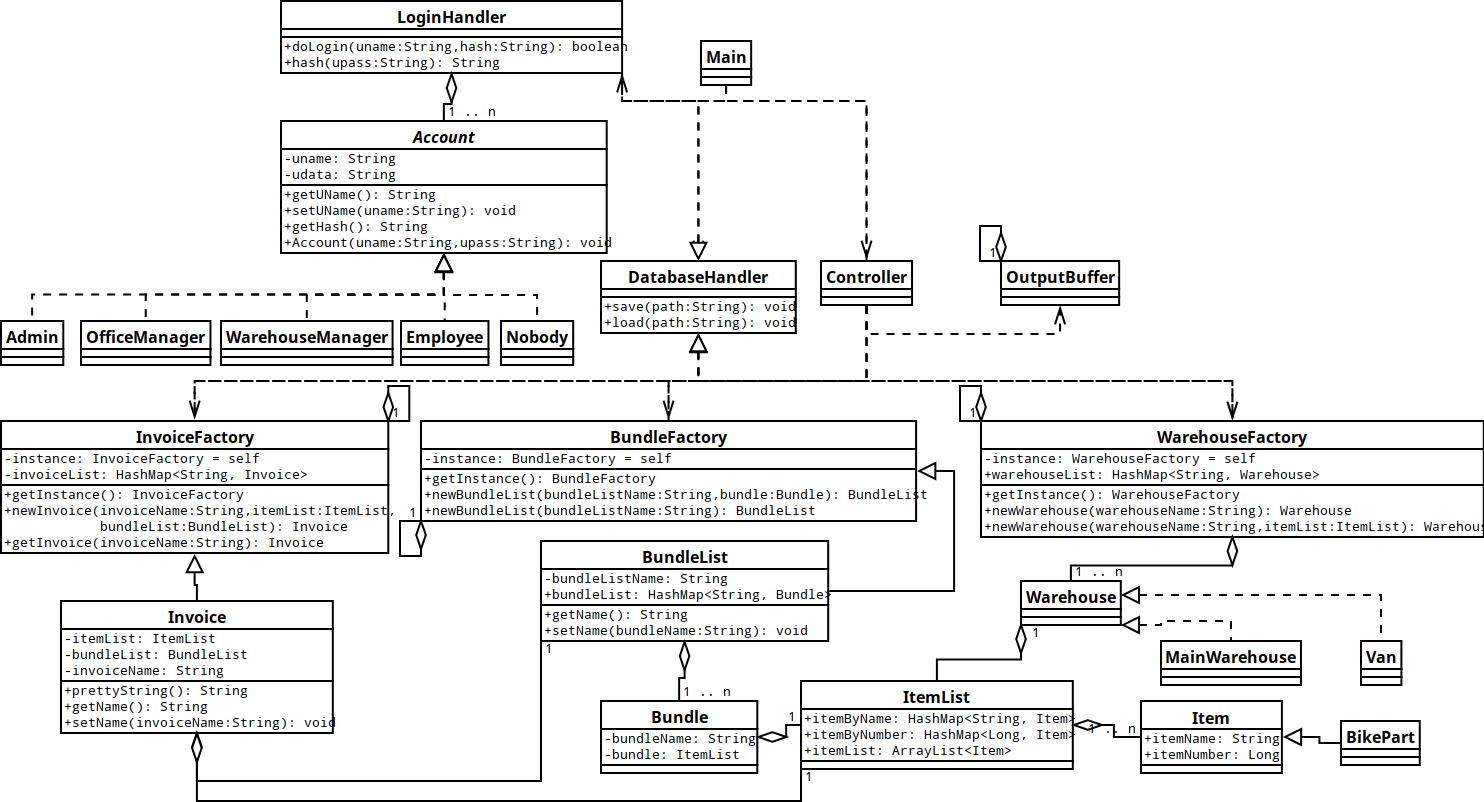
\includegraphics[width=\textwidth,height=\textheight,keepaspectratio]{overview.png}
%  \caption{Class hierarchy.}
%\end{sidewaysfigure}

%\begin{sidewaysfigure}[ht]
%  \centering
%    \includegraphics[scale=0.24,keepaspectratio]{sasequence.png}
%  \caption{Sequence to conduct a sale.}
%\end{sidewaysfigure}

%\begin{figure}[h]
%  \centering
%    \includegraphics[scale=0.5,keepaspectratio]{wmsequence.png}
%  \caption{Warehouse manager use cases.}
%\end{figure}

%\begin{figure}[h]
%  \centering
%    \includegraphics[scale=0.5,keepaspectratio]{ui.png}
%  \caption{The JavaFX UI for the project.}
%\end{figure}

\end{document}
